%\documentclass[draft]{beamer} %temporary render
\documentclass{beamer} %final render

\usepackage[french]{babel} 	%utilisation des
\usepackage[T1]{fontenc} 	%caracteres
\usepackage[utf8]{inputenc} 	%francais
\usepackage{graphicx}
\usepackage{color}
\usepackage{ccaption}
\usepackage{fancyvrb}
\usepackage{verbatim}
\usepackage{float}
\usepackage{csquotes}	%pour les citations
\usetheme{Frankfurt}
\usepackage{marvosym} % \MVRIGHTarrow
\usepackage{listings}
\usepackage{float}


\AtBeginSection[] 	%va permettre fl'affichage du sommaire avant
{					%chaque vouvelle partie
  \begin{frame}
    \frametitle{Plan}
    \tableofcontents[currentsection, hideothersubsections]
  \end{frame} 
}

\setbeamertemplate{navigation symbols}{}
\setbeamertemplate{footline}[frame number]
\setbeamercolor{footline}{fg=gray,bg=black}

\makeatletter
\newcommand\titlegraphicii[1]{\def\inserttitlegraphicii{#1}}
\titlegraphicii{}
\setbeamertemplate{title page}
{
  \vbox{}
   {\usebeamercolor[fg]{titlegraphic}\inserttitlegraphic\hfill\inserttitlegraphicii\par}
  \begin{centering}
    \begin{beamercolorbox}[sep=8pt,center]{institute}
      \insertinstitute
    \end{beamercolorbox}
    \begin{beamercolorbox}[sep=8pt,center]{title}
      \usebeamerfont{title}\inserttitle\par%
      \ifx\insertsubtitle\@empty%
      \else%
        \vskip0.25em%
        {\usebeamerfont{subtitle}\usebeamercolor[fg]{subtitle}\insertsubtitle\par}%
      \fi%     
    \end{beamercolorbox}%
    \vskip1em\par
    \begin{beamercolorbox}[sep=8pt,center]{author}
      \usebeamerfont{author}\insertauthor
    \end{beamercolorbox}
    \begin{beamercolorbox}[sep=8pt,center]{date}
      \usebeamerfont{date}\insertdate
    \end{beamercolorbox}%\vskip0.5em
  \end{centering}
  %\vfill
}
\makeatother
\author{Benjamin BARBESANGE et Benoît GARCON}
\title{Soutenance de Projet Ingénieur 3ème Année}
\subtitle{WatchDogZZ - Suivi de personnes dans les bâtiments}
%\institute{Siemens Industry Software\\ISIMA}
\date{Projet de 120h\\Soutenu le 21 Mars 2017}
% \titlegraphicii{\includegraphics[height=5mm]{watchdogzz.png}}
\titlegraphic{
\includegraphics[height=5mm]{isima.png}}

\logo{
\includegraphics[height=10mm]{logo.png}} %le logo en bas a droite

\begin{document}

	\begin{frame} %frame de titre
		\maketitle
    \vspace*{1cm}
    \footnotesize
    \begin{tabular}{ll}
      Tuteur projet &: Pierre COLOMB\\
      Référente ISIMA &: Eva HASSINGER
    \end{tabular}
	\end{frame}

%---------- Introduction

  \begin{frame}{Introduction}
    
    \begin{block}{Contexte}
      \begin{itemize}
        \item Proposition personnelle
        \item Domaine du tracking
        \item Nouvelles technologies
      \end{itemize}
    \end{block}

    \pause

    \begin{exampleblock}{Applications}
      \begin{itemize}
        \item Secourisme
        \item Sécurité
        \item Optimisation de déplacements
        \item Analyse des déplacements dans un bâtiment
      \end{itemize}
    \end{exampleblock}

    \pause

    \begin{alertblock}{Objectifs}
      \begin{itemize}
        \item Suivi des personnes en \textbf{temps réel}
        \item Architecture \textbf{simple} et \textbf{modulaire}
      \end{itemize}
    \end{alertblock}

  \end{frame}

%---------- Plan

  \begin{frame}{Plan}
    \tableofcontents
  \end{frame}

%---------- Etude

  \section{Présentation du projet}
  \begin{frame}{\secname}
    \begin{center}
      Carte du Marauder Harry Potter.
    \end{center}

    \begin{block}{Objectifs}
      \begin{itemize}
        \item Visualiser un bâtiment
        \item Visualiser les personnes
        \item Opérations auxiliaires
        \begin{itemize}
          \item Partager sa position
          \item Marqueurs personnalisés
          \item Itinéraires
        \end{itemize}
        \item Données à caractère personnel
      \end{itemize}
    \end{block}
    
    \pause

    \begin{alertblock}{Contraintes}
      \begin{itemize}
        \item Solution évolutive
        \item Implémentation d'une base
        \item Constante amélioration (non régression)
      \end{itemize}
    \end{alertblock}
    
  \end{frame}


  \subsection{Analyse de l'existant}
  \begin{frame}{\subsecname}
    \begin{block}{Méthodes de localisation}
      \begin{itemize}
        \item Intentionnelle
        \item Automatique
        \item \textbf{Open data}
      \end{itemize}  
    \end{block}
    
    \begin{block}{Géolocalisation}
      \begin{itemize}
        \item GPS intégré
        \item Smart*, Google Glass
        \item Suit les déplacements de l'utilisateur
      \end{itemize}
    \end{block}

    \pause

    \begin{alertblock}{Localiser des personnes dans des bâtiments ?}
      Pas de solution, nous devons créer la nôtre
    \end{alertblock}
    
  \end{frame}

  \subsection{Architecture proposée}
  \begin{frame}{\subsecname}

    \begin{columns}
      \begin{column}{0.5\textwidth}
        \begin{exampleblock}{Objectif}
          \begin{itemize}
            \item Implémenter un service web
            \item Architecture en 2 parties
            \begin{itemize}
              \item Client mobile
              \item Service web
            \end{itemize}
          \end{itemize}
        \end{exampleblock}
      \end{column}
      \begin{column}{0.5\textwidth}
        \begin{figure}
        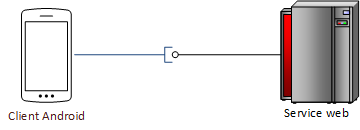
\includegraphics[width=\linewidth, height=\textheight, keepaspectratio]{archi_finale.png}
        \caption{Architecture proposée}
        \end{figure}
      \end{column}
    \end{columns}

    \pause

    \begin{block}{Répartition des tâches}
      \begin{itemize}
        \item Benoît : Client mobile
        \item Benjamin : Service web
      \end{itemize}
    \end{block}
  \end{frame}

  \subsection{Spécifications}
  \begin{frame}{\subsecname}
    \begin{block}{Service web}
      \begin{itemize}
        \item REST
        \item Stocker et distribuer des données
      \end{itemize}
    \end{block}

    \pause

    \begin{alertblock}{Fonctionnalités requises}
      \begin{itemize}
        \item Connecter / déconnecter l'utilisateur du service
        \item Fournir la liste des personnes connectées
        \item Fournir la position des utilisateurs
        \item Mettre à jour la position d'un utilisateur
      \end{itemize}
    \end{alertblock}

    \pause

    \begin{exampleblock}{Fonctionnalités supplémentaires}
      \begin{itemize}
        \item Fournir un historique de positions
        \item Calculer un itinéraire
        \item Partager sa position (sms, mail)
      \end{itemize}
    \end{exampleblock}

  \end{frame}

  \begin{frame}{\subsecname}
    \begin{block}{Client mobile}
      \begin{itemize}
        \item \textbf{Un client} du service
        \item Mobile : \textbf{portabilité}
        \item But : servir d'\textbf{interface} aux utilisateurs finaux
      \end{itemize}
    \end{block}

    \pause

    \begin{alertblock}{Fonctionnalités requises}
      \begin{itemize}
        \item Gérer un utilisateur
        \item Consommer le service
        \item Répondre à des critères d'\textbf{utilisabilité} et de \textbf{performances}
      \end{itemize}
    \end{alertblock}

    \pause

    \begin{exampleblock}{Fonctionnalités supplémentaires}
      \begin{itemize}
        \item Visualiser une carte en 3D
        \item Visualier en réalité virtuelle
        \item Ajouter des informations personnalisées
      \end{itemize}
    \end{exampleblock}

  \end{frame}


  \section{Réalisation de la solution}
  \subsection{Technologies transverses}
  \begin{frame}{\subsecname}
    \begin{block}{Travis CI}
      \begin{itemize}
        \item Intégration continue
        \item \textbf{Tests} et \textbf{déploiements} automatiques
      \end{itemize}
    \end{block}

    \begin{block}{GitHub}
      \begin{itemize}
        \item \textbf{Versionner} le code source
        \item \textbf{Planifier} et \textbf{assigner} des tâches
        \item Recenser les bugs
      \end{itemize}
    \end{block}
    
  \end{frame}

  \subsection{Technologies mobile}
  \begin{frame}{\subsecname}
  \begin{columns}
    \begin{column}{0.62\textwidth}
      \begin{block}{Android}
        \begin{itemize}
          \item Choix personnel
          \item Android studio
          \item Framework (version > 12)
          \item Gestion du réseau
          \begin{itemize}
            \item Volley
            \item Picasso
          \end{itemize}
          \item Bibliothèque graphique : OpenGL ES
        \end{itemize}
      \end{block}
      
    \end{column}
    \begin{column}{0.38\textwidth}
      \begin{figure}
        
\includegraphics[height=0.25\textheight, keepaspectratio]{android.png}
      \end{figure}
      \begin{figure}
        
\includegraphics[width=\linewidth, height=\textheight, keepaspectratio]{opengl.png}
      \end{figure}
    \end{column}
  \end{columns}
    
  \end{frame}

  \subsection{Réalisation mobile}
  \begin{frame}{\subsecname}
      \begin{center}
        Architecture MVC
        \begin{figure}
        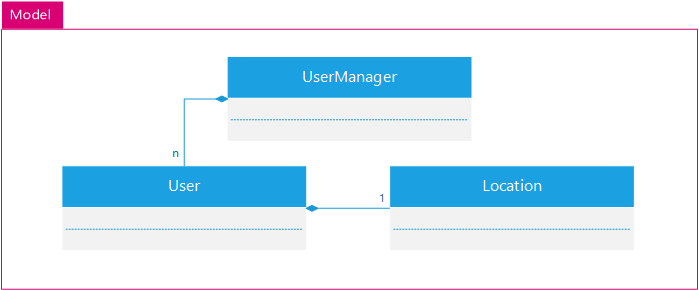
\includegraphics[width=0.58\linewidth, height=\textheight, keepaspectratio]{android-model.png}
        \end{figure}
      \end{center}

      \vspace*{-8mm}

      \begin{columns}
        \begin{column}{0.58\textwidth}
          \begin{figure}
          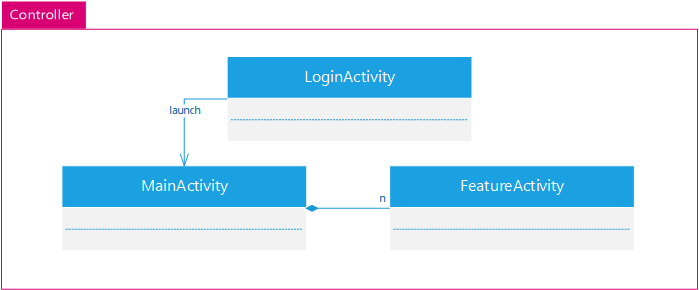
\includegraphics[width=\linewidth, height=\textheight, keepaspectratio]{android-controller.png}
          \end{figure}
        \end{column}
        \begin{column}{0.58\textwidth}
          \begin{figure}
          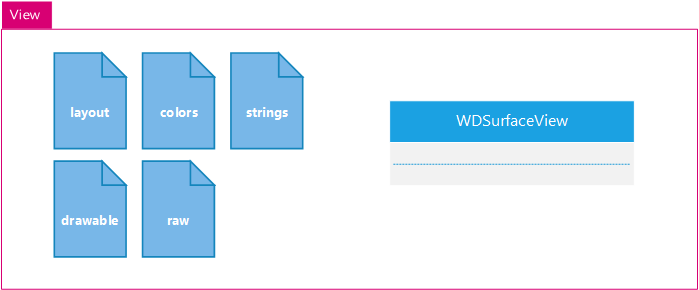
\includegraphics[width=\linewidth, height=\textheight, keepaspectratio]{android-view.png}
          \end{figure}
        \end{column}
      \end{columns}

  \end{frame}

  \begin{frame}{\subsecname}
    \begin{block}{Composition de l'application}
      \begin{itemize}
        \item 3 activités
        \begin{itemize}
          \item Unité d'action
          \item Des fragments
        \end{itemize}
      \end{itemize}
    \end{block}

    \begin{block}{Communications}
      \begin{itemize}
        \item Utilisation de services asynchrones
        \item Communication réseau
      \end{itemize}
    \end{block}
    
  \end{frame}

  \subsection{Technologies serveur}
  \begin{frame}{\subsecname}

    \begin{columns}
      \begin{column}{0.58\textwidth}
        \begin{block}{Technologies}
          \begin{itemize}
            \item Framework NodeJS
            \item Ajout de paquets NPM
            \begin{itemize}
              \item Express : serveur web
              \item Jasmine : tests par specs
              \item MongoDB : gestion de la base
              \item Winston : système de log
            \end{itemize}
            \item MongoDB : base de données
          \end{itemize}
        \end{block}
        
      \end{column}
      \begin{column}{0.38\textwidth}
        \begin{figure}
        
\includegraphics[width=\linewidth, height=\textheight, keepaspectratio]{nodeexpress.png}
        \end{figure}
        \begin{figure}
          
\includegraphics[width=\linewidth, height=0.1\textheight, keepaspectratio]{npm.png}
        \end{figure}
      \end{column}
    \end{columns}

    \pause

    \begin{exampleblock}{Services ajoutés}
      \begin{itemize}
        \item DNS et DynDNS
        \item Https avec Letsencrypt
        \item Log d'erreurs
      \end{itemize}
    \end{exampleblock}

  \end{frame}

  \subsection{Réalisation serveur}
  \begin{frame}{\subsecname}
    \vspace*{-2mm}
    \begin{figure}
      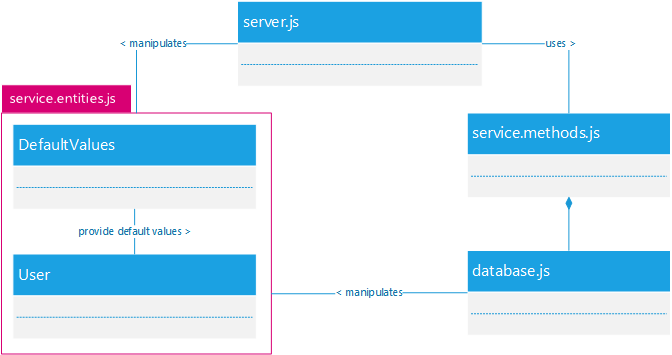
\includegraphics[width=0.8\linewidth, height=\textheight, keepaspectratio]{architecture-service-web-simple.png}
    \end{figure}

    \pause

    \begin{block}{Description}
      \begin{itemize}
        \item server.js : code \textbf{serveur} et gestion de \textbf{requêtes} \pause
        \item service.entities.js : gestion des \textbf{entités} et \textbf{valeurs par défaut} \pause
        \item service.methods.js : wrapper l'utilisation de la base de données \pause
        \item database.js : code de gestion \textbf{MongoDB}
      \end{itemize}
    \end{block}
  \end{frame}

  \section{Résultats}
  \subsection{Service à disposition}
  \begin{frame}[fragile]{\subsecname}

    \begin{block}{URLs mises en place}
      \begin{itemize}
        \item POST /login : se connecter
        \item POST /logout : se déconnecter
        \item GET /who : lister les personnes connectées
        \item POST /where : mettre à jour sa position
        \item GET /where : obtenir les positions des utilisateurs
      \end{itemize}
    \end{block}

    \pause

    \begin{exampleblock}{Exemple de corps de requête (POST /where)}
      \begin{verbatim}
        {
            "token": "1A2Z3E4R5T6Y7U8I9O0P",
            "location": [
                1.0, 2.0, 3.0
            ]
        }
      \end{verbatim}
    \end{exampleblock}

\end{frame}
% ne pas indenter ce \end

  \subsection{Client Android}
  \begin{frame}{\subsecname}
    \begin{block}{Fonctionnalités}
      \begin{itemize}
        \item Localisation
        \begin{itemize}
          \item Affichage des utilisateurs connectés
          \item Synchronisation de la position avec le serveur
          \item Définition des points d'intérêt
          \item Affichage 3D
        \end{itemize}

        \pause

        \item Communication
        \begin{itemize}
          \item Authentification Google
          \item Partage de position
        \end{itemize}
      \end{itemize}
    \end{block}
    
  \end{frame}

  \begin{frame}[T]{\subsecname}
    \begin{center}
      Quelques écrans
    \end{center}

    % \vspace*{-1cm}

    \begin{columns}[T]
      \begin{column}{0.5\textwidth}
        \begin{figure}
          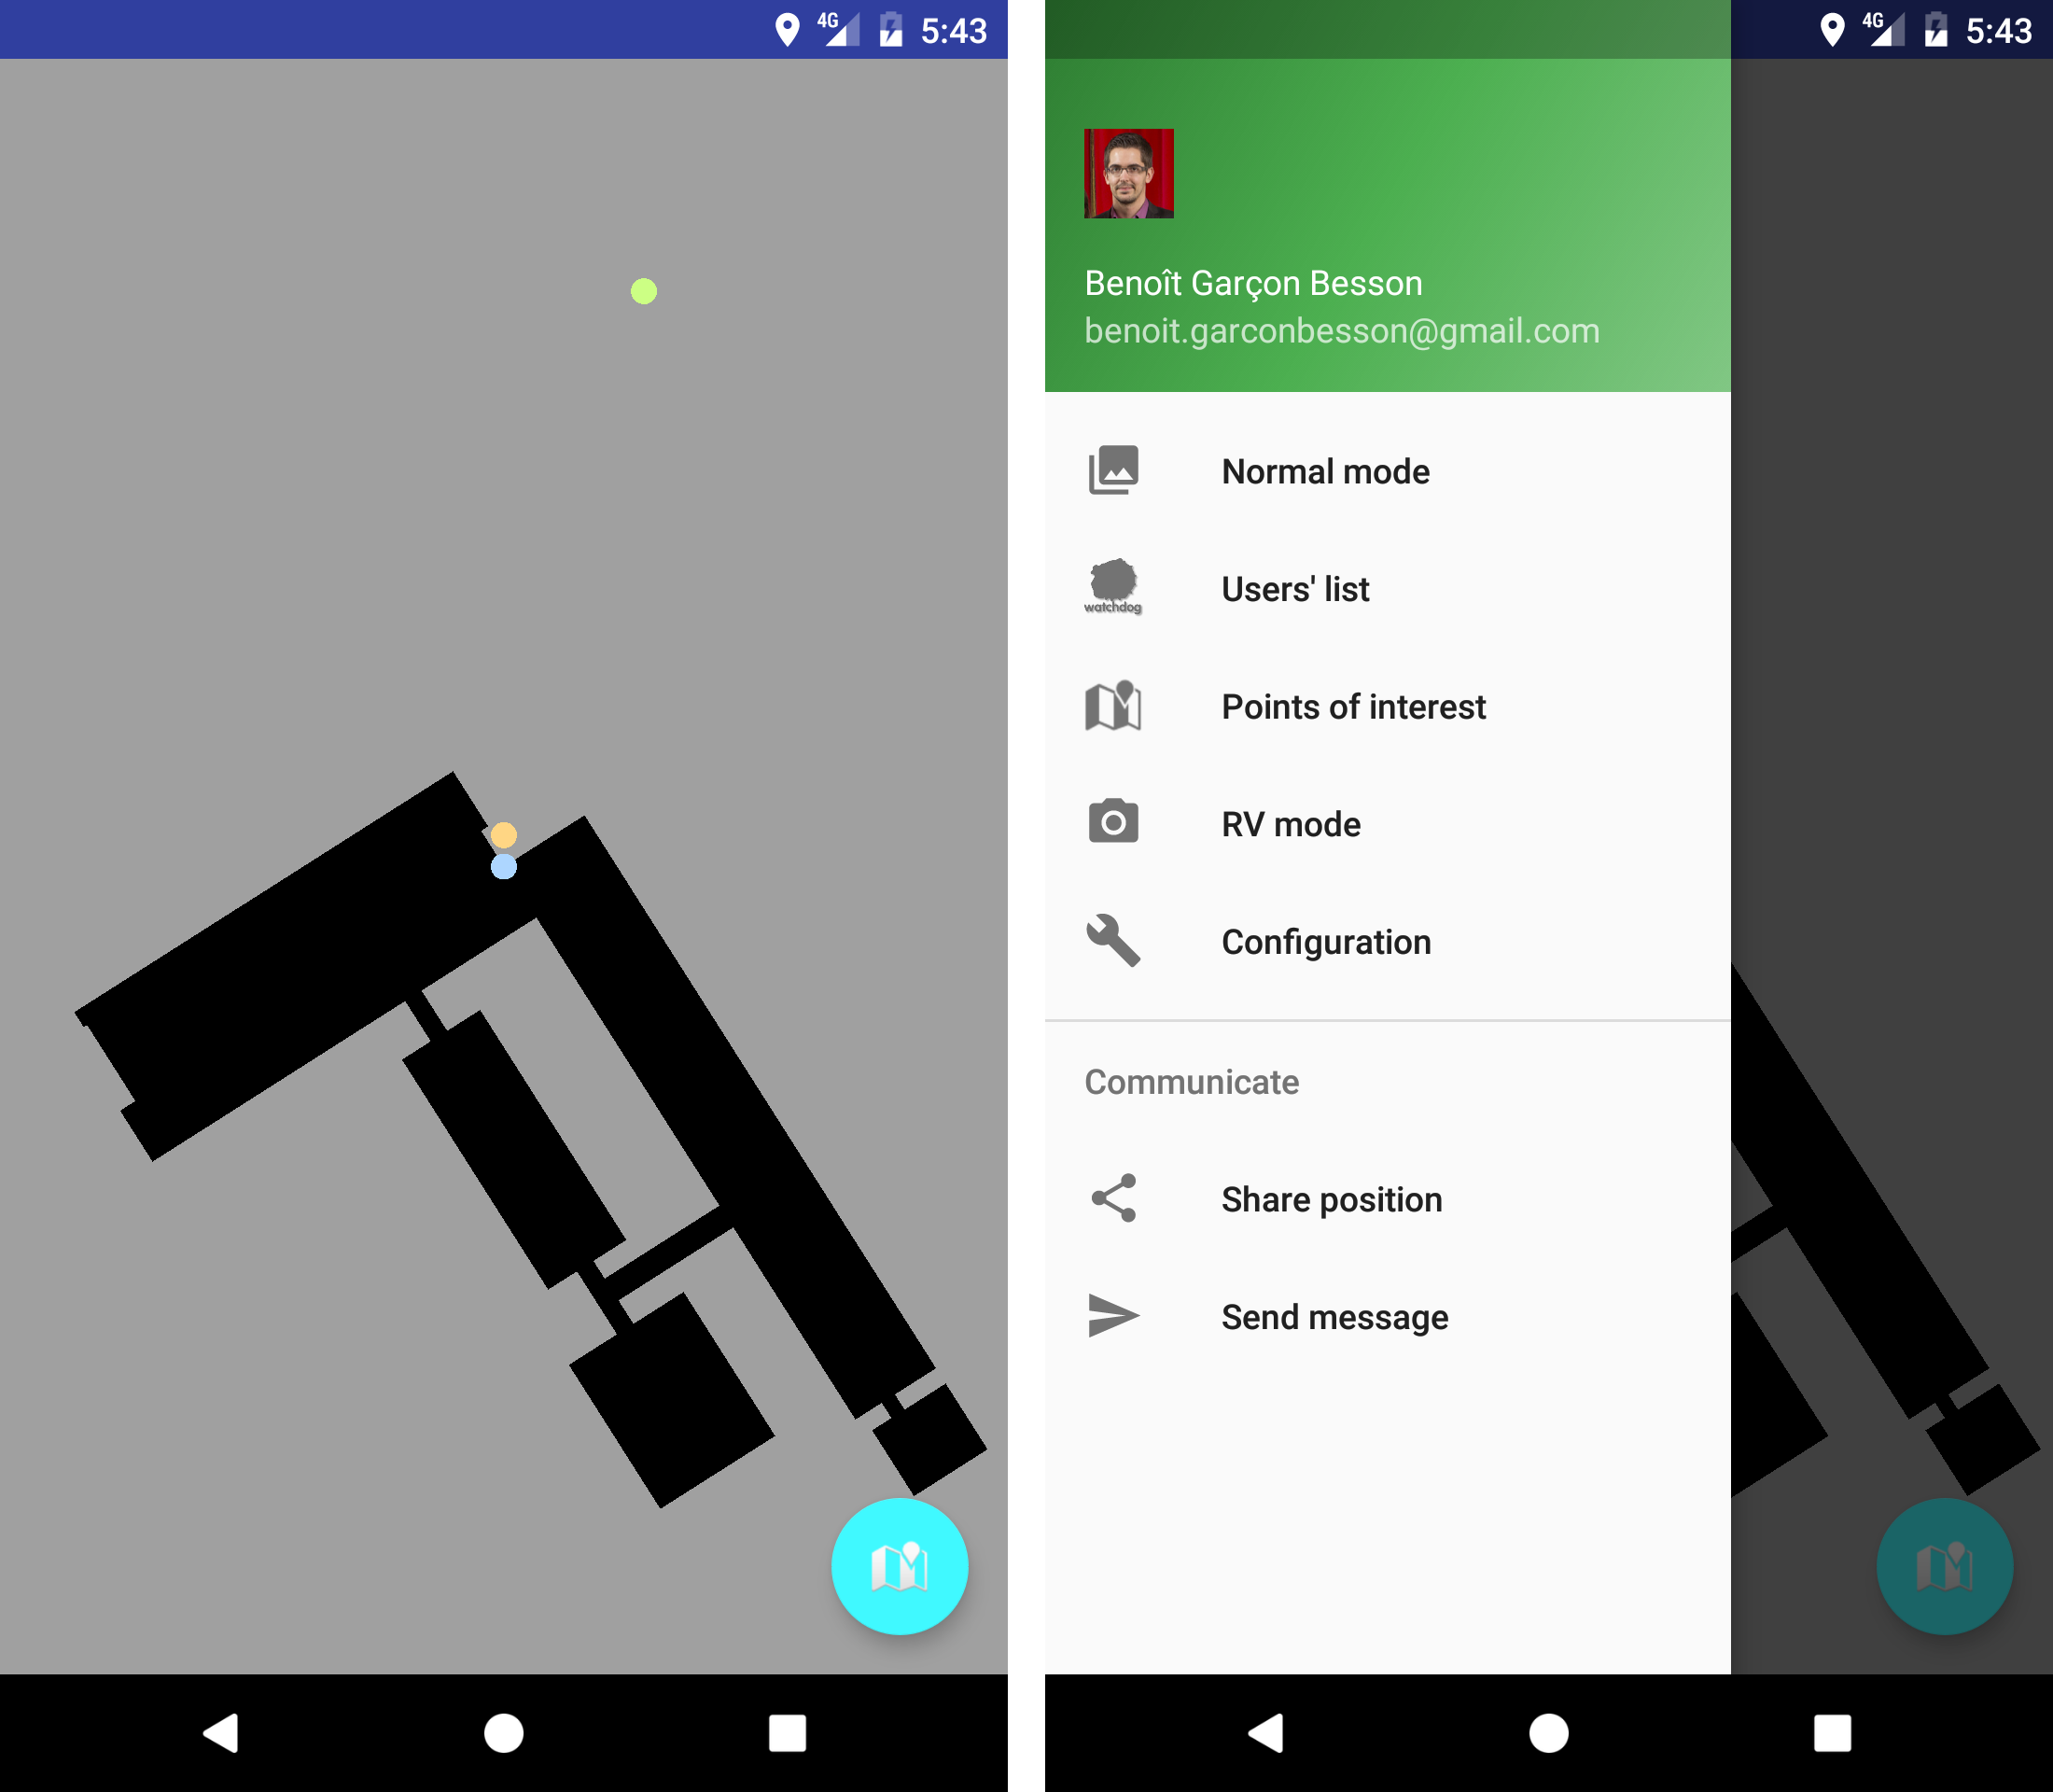
\includegraphics[width=\linewidth, height=\textheight, keepaspectratio]{screen2.png}
          \caption{Visualisation de la carte et menu latéral}
        \end{figure}
      \end{column}
      \begin{column}{0.50\textwidth}
        \begin{figure}
          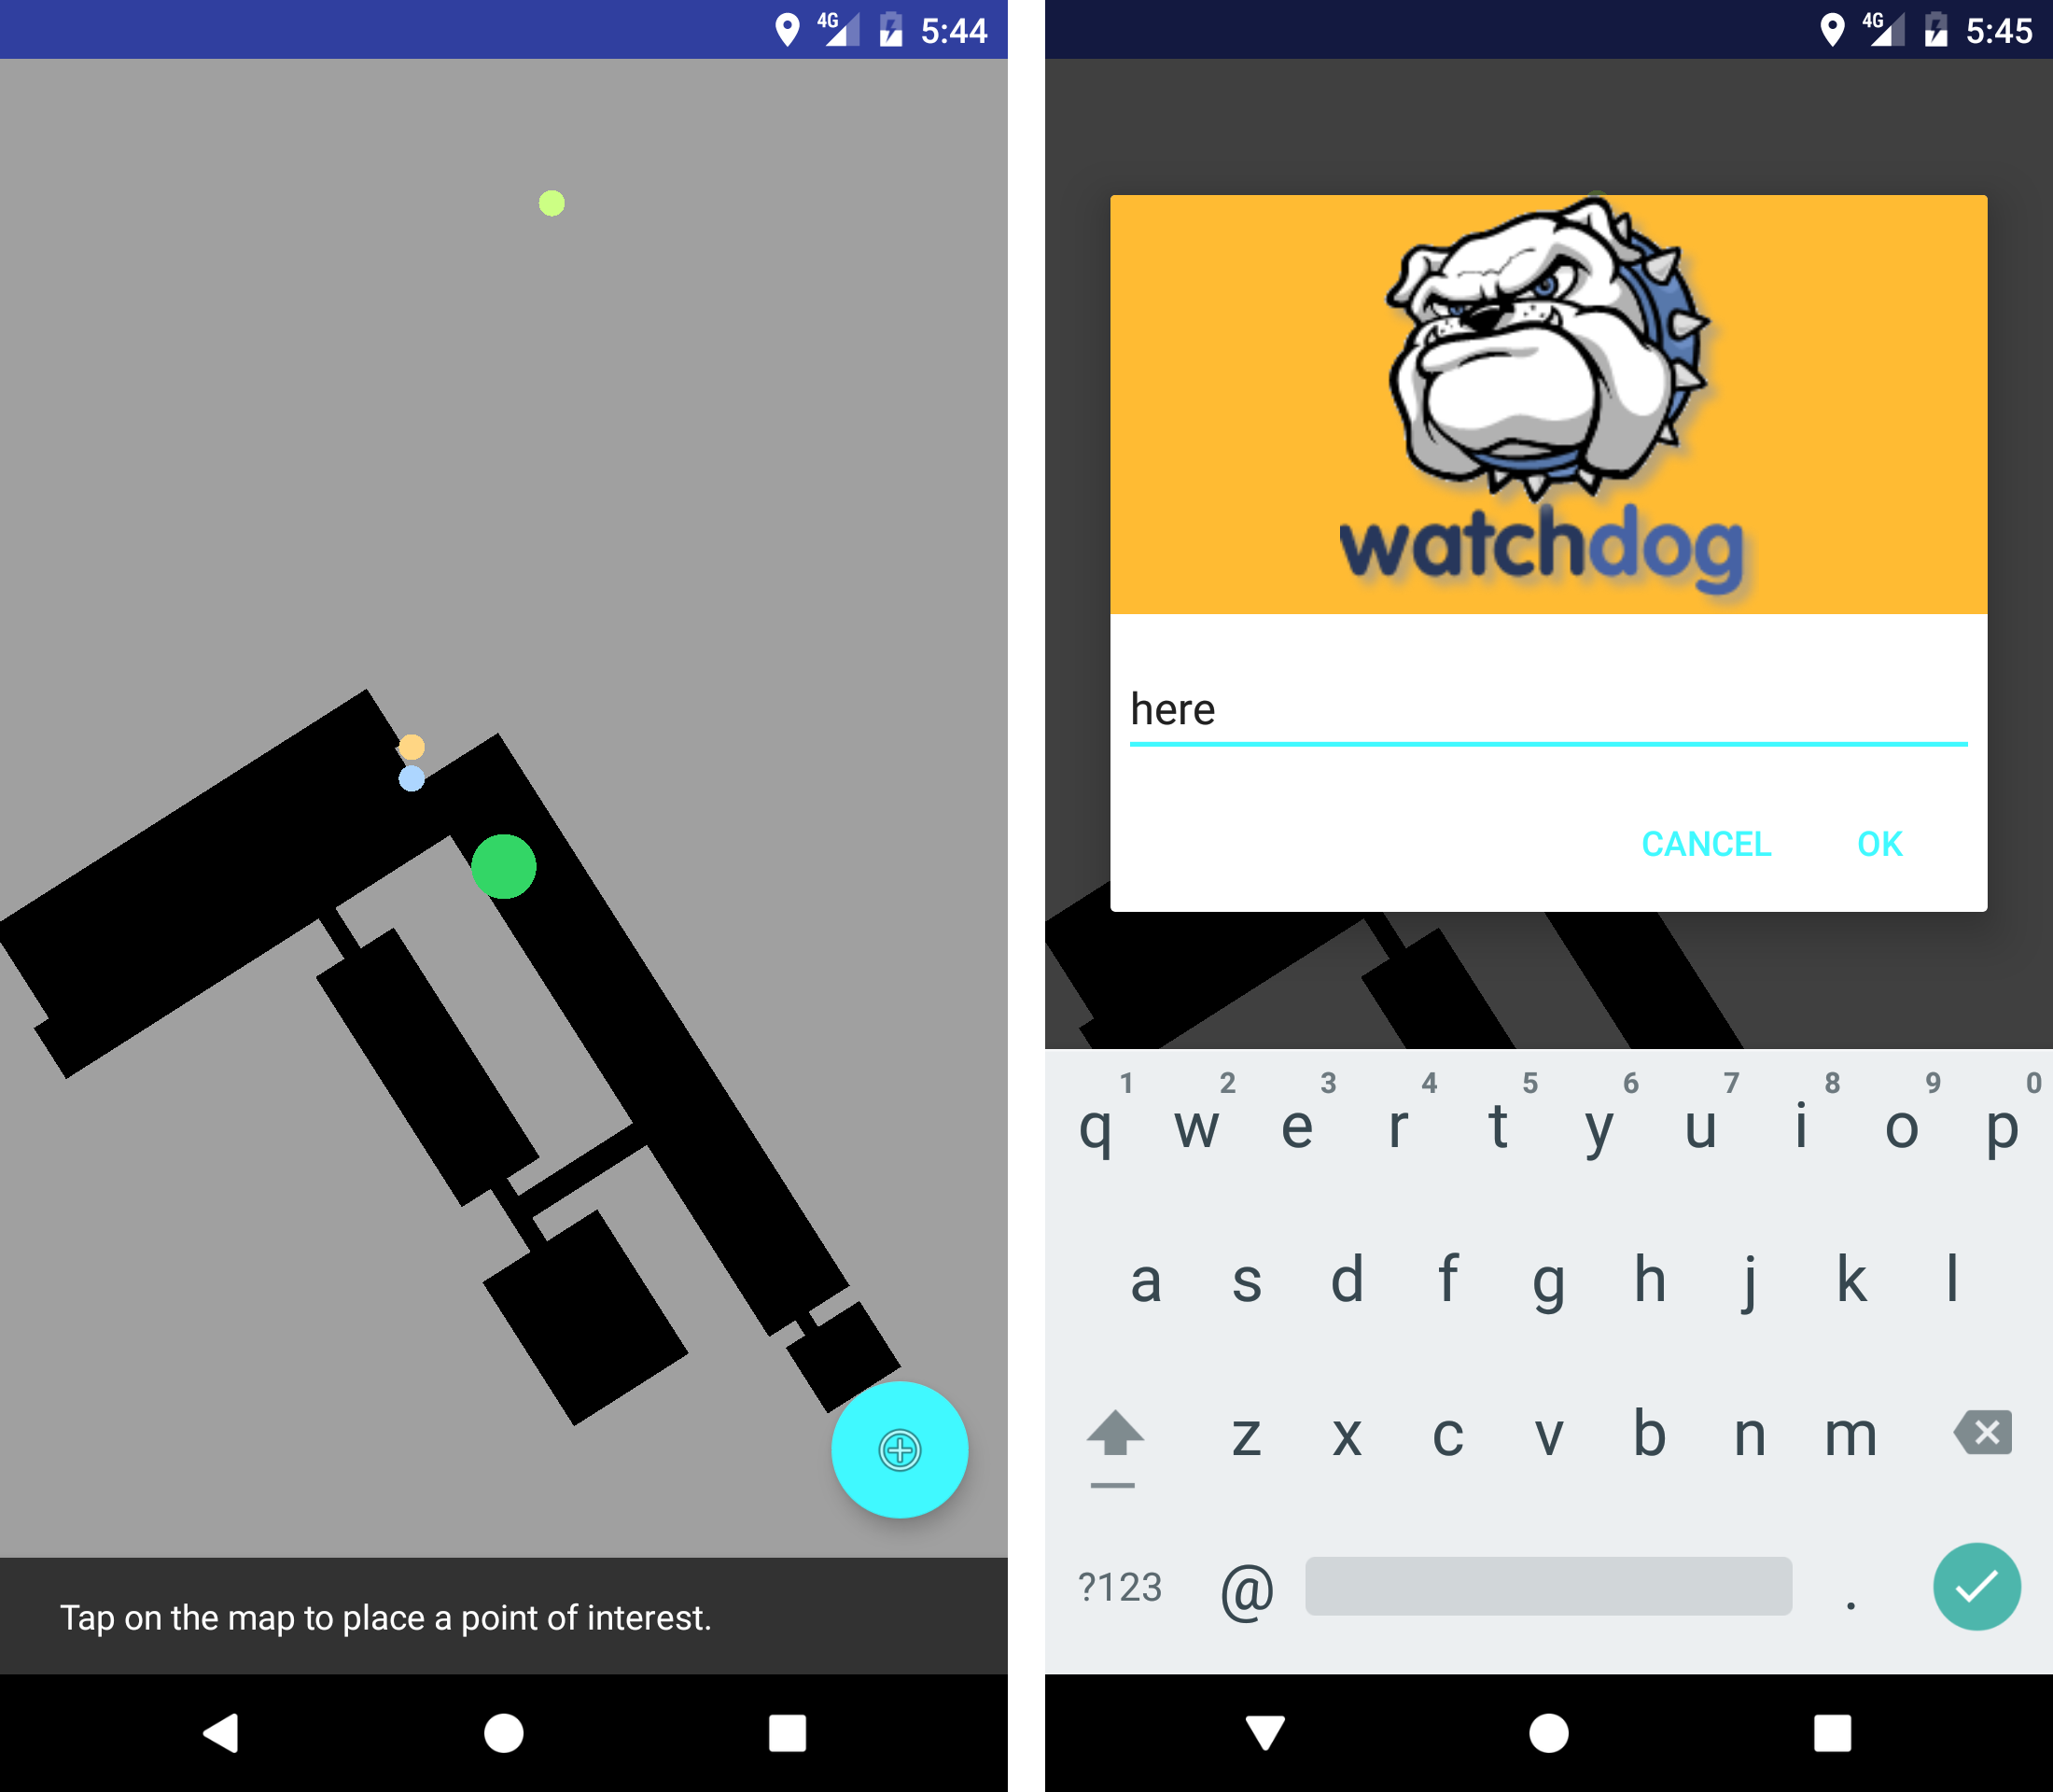
\includegraphics[width=\linewidth, height=\textheight, keepaspectratio]{screen4.png}
          \caption{Ajout d'un point d'intérêt sur la carte}
        \end{figure}
      \end{column}
    \end{columns}
  \end{frame}

  \subsection{Améliorations possibles}
  \begin{frame}{\subsecname}
    \begin{block}{Client}
      \begin{itemize}
        \item Amélioration de l'interface
        \item Paramétrage de l'utilisateur
        \item Mode réalité virtuelle : Google cardboard
        \item Gestion des étages : calibration
      \end{itemize}
    \end{block}

    \pause

    \begin{block}{Serveur}
    \begin{itemize}
      \item Calcul d'itinéraires
      \item Gestion des logs
      \item Alertes automatiques
    \end{itemize}
    \end{block}
    
  \end{frame}
  
%---------- Conclusion

  \section{Conclusion}
  \begin{frame}{\secname}
      \begin{block}{Rappels}
        \begin{itemize}
          \item Suivi de personnes
          \item Service web : réceptionner et traiter des données
          \item Client : fournir et demander des données
        \end{itemize}
      \end{block}

      \pause

      \begin{alertblock}{Points négatifs}
        \begin{itemize}
          \item Client uniquement android : iOs, Windows Universal, Site web
          \item Déploiement sur le cloud
        \end{itemize}
      \end{alertblock}

  \end{frame}

  \begin{frame}{\secname}
    \begin{exampleblock}{Points positifs}
        \begin{itemize}
          \item Architecture modulaire
          \item Processus d'intégration
          \begin{itemize}
            \item Intégration continue
            \item Tests automatiques
            \item Déploiement automatique
          \end{itemize}
        \end{itemize}
      \end{exampleblock}

      \pause

      \begin{block}{Perspectives}
        \begin{itemize}
          \item Améliorations possibles
          \item Projet accessible librement sur GitHub
          \item Tout le monde peut y contribuer
        \end{itemize}
      \end{block}
  \end{frame}

%---------- Remerciement

  \begin{frame}{Fin}
    \begin{center}
      \huge
      Merci de votre attention.

      \begin{figure}
        
\includegraphics[width=\linewidth, height=0.6\textheight, keepaspectratio]{logo.png}
      \end{figure}
    \end{center}
  \end{frame}

\end{document} %finished!
